
\chapter{A closer look at Bro's Reassemblers} \label{chap:deeper}

It is now clear that, with reassembly playing such an important part in the analysis of packets' payloads, it is necessary to allow Bro to reassemble data from multiple streams within the Engine. In order to assess what is necessary to achieve this, we will now examine in detail how Bro performs reassembly of regular TCP. To do this, we will explain how Bro manages individual data streams, then how it handles reassembly on streams using TCP.

\section{Identifying Streams}
As we have already mentioned, Bro takes a stream-oriented approach at analyzing traffic. This means that all the packets that belong to the same connection are processed together as a single coherent data stream. In order to do this, Bro goes through a number of steps in order to uniquely identify all the connections that it sees. Since the software aims at inspecting the payload, information that is purely routing-related is mostly ignored. To this end, removing tunneling information and MPLS labels is one of the first steps. Once this is done, Bro can then move on to the next layers of the packet. In the case that interests us, Bro will then assess that the packet uses either IPv4 or IPv6. It will then perform reassembly of fragmented IP packets, if necessary, before moving on to the transport layer. \\

By continuing the parsing of the packet headers, Bro will split up incoming packets according to the transport protocol in use. Once it is determined, the Engine can properly extract the Addresses from the IP header and, in the case of TCP, the port numbers. Up until this point, Bro does not maintain any long-term state about the packet, simply relying on temporary storage such as buffers for the de-fragmentation. With the four address and port values available, Bro will now start uniquely identifying connections. Connections are represented by a complex Conn data structure containing information about the stream, as well as being in charge of maintaining the analyzer tree that will be used and performing the subsequent analysis of the connection's traffic. The connection manager keeps dictionaries containing all the Conns of a given protocol. We create a Conn ID structure containing the four-tuple along with a boolean indicating the direction of the connection, and the hashed value of this data structure serves as a key in the dictionaries. It is important to note that Bro therefore limits the distinction of different connections to these five values.\\

For each incoming packet, the Conn ID is calculated and hashed, and the resulting key is used in a lookup in the corresponding dictionary. If a match is found, the packet is treated by the match's Conn structure. If the dictionary does not contain an entry for the key, a new Conn is created and added. It is also at this point that the connection's analyzer tree is initialized. In our case, the TCP analyzer is selected as root, given that this is the transport protocol in use. Each connection will dispose of its own instantiation of the required analyzers. To complement the analyzers, a PIA is also initialized. The PIA is the mechanism responsible for dynamically detecting which application-layer protocols are used within the connection, and will therefore build or prune the analyzer tree as the connection progresses. However, the root analyzer will not change, given that the connection will keep using TCP throughout its lifetime. The child analyzers do not concern us and we will therefore not go into detail on how the PIA works.\\

At this point, we have a Conn structure unique to the connection using the address, port, and direction 5-tuple. This Conn is stored within the TCP connection dictionary of Bro's session manager, allowing future packets from the connection to be matched straight to it. The structure also contains an analyzer tree rooted at a TCP analyzer. This TCP analyzer is where we performed modifications during our first attempt. In order to go further, we will now see how this analyzer reconstructs the TCP stream that it is in charge of.

\section{Bro's TCP Endpoints and Reassemblers}

Bro's TCP analyzers use several supporting classes in order to process TCP traffic both efficiently, and in a way similar to how the actual end hosts proceed. One such component is the TCP Endpoint. When a new analyzer is instantiated, it immediately creates two TCP Endpoints which each represent one of the two hosts involved in the connection. Since each host has its own parameters and receives a different data stream, this is a natural way to proceed. In practice, each TCP Endpoint's primary function is to keep track of the host's state with regards to the connection. It will, for example, keep track of whether or not the host considers the connection established or terminated, as well as the sequence and acknowledgment numbers that it has seen and is expecting. \\

Since the TCP Endpoints are already tracking the sequence and acknowledgment numbers, this is the ideal place to perform reassembly. Additionally, each host's traffic must be reassembled separately and the distinction is already done at this point. Therefore, the TCP Reassemblers are added as elements of the TCP Endpoints. The TCP Reassembler itself will be in charge of ensuring that only contiguous data blocks are sent to the analyzer's children. \\

Now, whenever a packet arrives on the connection, the TCP analyzer will first determine which of its two endpoints sent it and to which one it is destined. At every point during the analysis of the TCP header, the analyzer can now notify its Endpoints of the changes that occurred. SYN or FIN flags will update the corresponding Endpoint's state. Acknowledgments and TCP payloads are explicitly transferred to the receiving Endpoint as well, allowing the corresponding values to be updated. The Endpoint itself does little with these last two elements, but in turn transfers them to its Reassembler. The Reassembler will then compare the incoming data's starting point to the data it has already delivered. If a gap of data is detected, the payload is buffered until the gap is filled. At that point, all the newly contiguous data can be delivered. The data itself is actually re-sent to the TCP Analyzer. Since the analyzer has already processed that data for any TCP-related information, it simply forwards it to its children analyzers. Figure \ref{pic:reassembly_data} shows how the data travels through the TCP analyzer to the different components of reassembly.


\begin{figure}[!t]
\centering
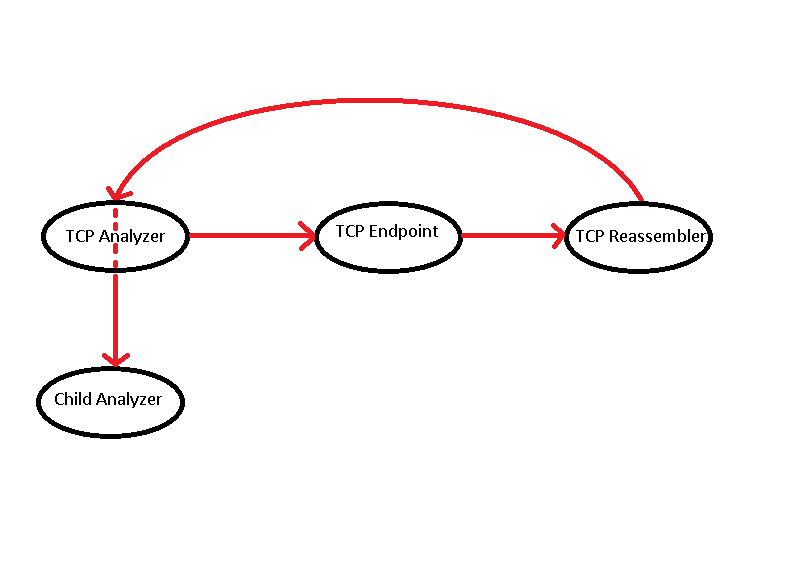
\includegraphics[scale = 0.6]{Figures/reassemblydata.png}
\caption{Data Path for reassembling TCP Data}
\label{pic:reassembly_data}
\end{figure}